% -*- TeX -*- -*- DE -*-

\chapter{Grundlagen}\label{ch:Grundlagen}
Hier wird kurz aufgezählt was erläutert wird. Mehr nicht. \
Es sollen hier nur Elemente erläutert werden, die für mindestens zwei der Methoden relevant sind.\
k-center greedy (PatchCore), Autoencoder (efficientad) oder Backpropagation (simplenet) also zB nicht.\

\section{Datensatz: MVTecAD\cite{mvtecad}}\label{sec:DatensatzMVTecAD}
Das \glqq MVTec Anomaly Detection Dataset\grqq{} (MVTec AD) ist ein am 6. Januar 2021 veröffentlichter, umfangreicher Datensatz für die Anomalieerkennung in Bildern. \
Dieser bildet die Evaluationsgrundlage aller hier in dieser Arbeit vorkommendene Entwicklungen und Methoden. \
Treibende Kraft hinter der Entwicklung des Datensatzes ist die MVTec Software GmbH, ein deutsches Unternehmen, das sich auf industrielle Bildverarbeitung spezialisiert hat. \
Dieser Datensatz ist entwickelt worden, um einen internationalen Benchmark zu schaffen, der die Entwicklung von Algorithmen für die Unüberwachte Anomalieerkennung in Bildern vorantreibt und Methoden quantitativ vergleichbar macht. \
Betrachtet man die Anzahl an Veröffentlichungen, beispielsweise auf \url{https://paperswithcode.com/sota/anomaly-detection-on-mvtec-ad}, fällt auf, dass seit der Veröffentlichung des Datensatzes \
immer mehr Methoden auf diesem Datensatz evaluiert werden. Waren es 2020 22 Veröffentlichungen stieg die Anzahl streng monoton bis auf bereits 80 im laufenden Jahr 2023 (Stand 11.10.2023). \\
Der Datensatz besteht aus insgesamt 5354 Bildern, die 15 verschiedene Klassen von Objekten enthalten. Die folgende Tabelle gibt einen Überblick über die Klassen und die Anzahl an Bildern pro Klasse. \
\begin{table}[h]
  \centering
  \begin{tabular}{|c|p{1.8cm}|p{1.8cm}|p{1.8cm}|p{1.8cm}|p{1.8cm}|p{1.8cm}|}
  \hline
  Category & \#Train & \#Test (good) & \#Test (defective) & \#Defect groups & \#Defect regions & Image side length  \\
  \hline
  Carpet & 280 & 28 & 89 & 5 & 97 & 1024 \\ 
  Grid & 264 & 21 & 57 & 5 & 170 & 1024 \\
  Leather & 245 & 32 & 92 & 5 & 99 & 1024 \\ 
  Tile & 230 & 33 & 84 & 5 & 86 & 840 \\
  Wood & 247 & 19 & 60 & 5 & 168 & 1024  \\ 
  Bottle & 209 & 20 & 63 & 3 & 68 & 900 \\
  Cable & 224 & 58 & 92 & 8 & 151 & 1024 \\ 
  Capsule & 219 & 23 & 109 & 5 & 114 & 1000 \\
  Hazelnut & 391 & 40 & 70 & 4 & 136 & 1024 \\ 
  Metal nut & 220 & 22 & 93 & 4 & 132 & 700 \\
  Pill & 267 & 26 & 141 & 7 & 245 & 800 \\ 
  Screw & 320 & 41 & 119 & 5 & 135 & 1024 \\
  Toothbrush & 60 & 12 & 30 & 1 & 66 & 1024 \\ 
  Transistor & 213 & 60 & 40 & 4 & 44 & 1024 \\
  Zipper & 240 & 32 & 119 & 7 & 177 & 1024 \\
  \hline
  Total & 3629 & 467 & 1258 & 73 & 1888 & - \\
  \hline
  \end{tabular}
  \caption{Übersicht über Anzahl an Bildern, Auflösung und Defektgruppen des Datensatzes}
  \label{tab:mvtecad_overview}
\end{table}
Diese 15 Klassen lassen sich in zehn Objektklassen und fünf Texturklassen unterteilen. Die fünf ersten Klassen der Tabelle (Carpet, Grid, Leather, Tile, Wood) sind Texturen bzw. Strukturen, \
die weiteren zehn Klassen (Bottle, Cable, Capsule, Hazelnut, Metal nut, Pill, Screw, Toothbrush, Transistor, Zipper) sind Objekte. \\
Wie bereits erwähnt, handelt es sich um einen Datensatz für Unüberwachte Anomaliedetekion, was sich daran erkennen lässt, dass in den Trainingsdaten ausschließlich Bilder ohne Defekte (nominal) enthalten sind. \
Die Testdaten sind in zwei Klassen unterteilt: \glqq Good\grqq{} und \glqq Defective\grqq{}. Zwar liegen in den meisten Fällen mehrere mögliche Defektklassen vor, die auch eindeutig gelabelt werden, allerdings \
handelt es sich um einen Binärklassifikationsdatensatz, was bedeutet, dass das Erkennen der Art des Defektes keine Zielstellung ist. Durch diese Vielzahl an Defekten kann aber eine gewisse Generalisierungsfähigkeit getestet werden. \\
Alle anomalen Testbilder habem eine pixelweise Annotation, die die Defekte markiert. Diese Annotationen sind in Form von Binärbildern gegeben, wobei die Pixel der Defekte mit $1$ und die Pixel der nominalen Regionen mit $0$ markiert sind. \
In dieser Arbeit liegt zwar der Fokus auf der Instanzklassifizierungsgenauigkeit und nicht auf der Segmentierung. Dennoch ist diese qualitativ hochwertige Annotation ein wohl wesentlicher Grund für die Beliebtheit des Datensatzes. \
Nicht nur lässt sich damit schlicht die Segmentierungsgenauigkeit testen, sondern der Vergleich einer von einer Methode zu einem Testbild festgestellte Anomaliekarte mit der Annotation ist ein wertvolles Werkzeug, \
um die Funktionsweise einer Methode zu verstehen und etwaige Schwachstellen zu identifizieren. \\
Anzumerken ist, dass es sich bei den vorliegenden Defekten um keine logischen Defekte handelt, sonder um lokale, strukturelle Abweichungen von der Norm. Die grundsätzliche Gestalt ist auch im Falle eines anomalen Bildes erhalten. \ 
Möchte man zum Beispiel ein Anomaliedetekionsverfahren entwickeln, das zu lang geratene oder stark gekrümmte Schrauben erkennt, so ist der Datensatz nicht optimal geeignet. Hierzu sei auf den neueren Datensatz aus dem Hause MVTec, \ 
MvTec LOCO AD verwiesen. \cite{mvtecadloco} Beisple für nominale und anomale Bilder aus dem Datensatz finden sich in Abbildung \ref{fig:mvtecad_examples}. \\
\begin{figure}[h]
  \centering
  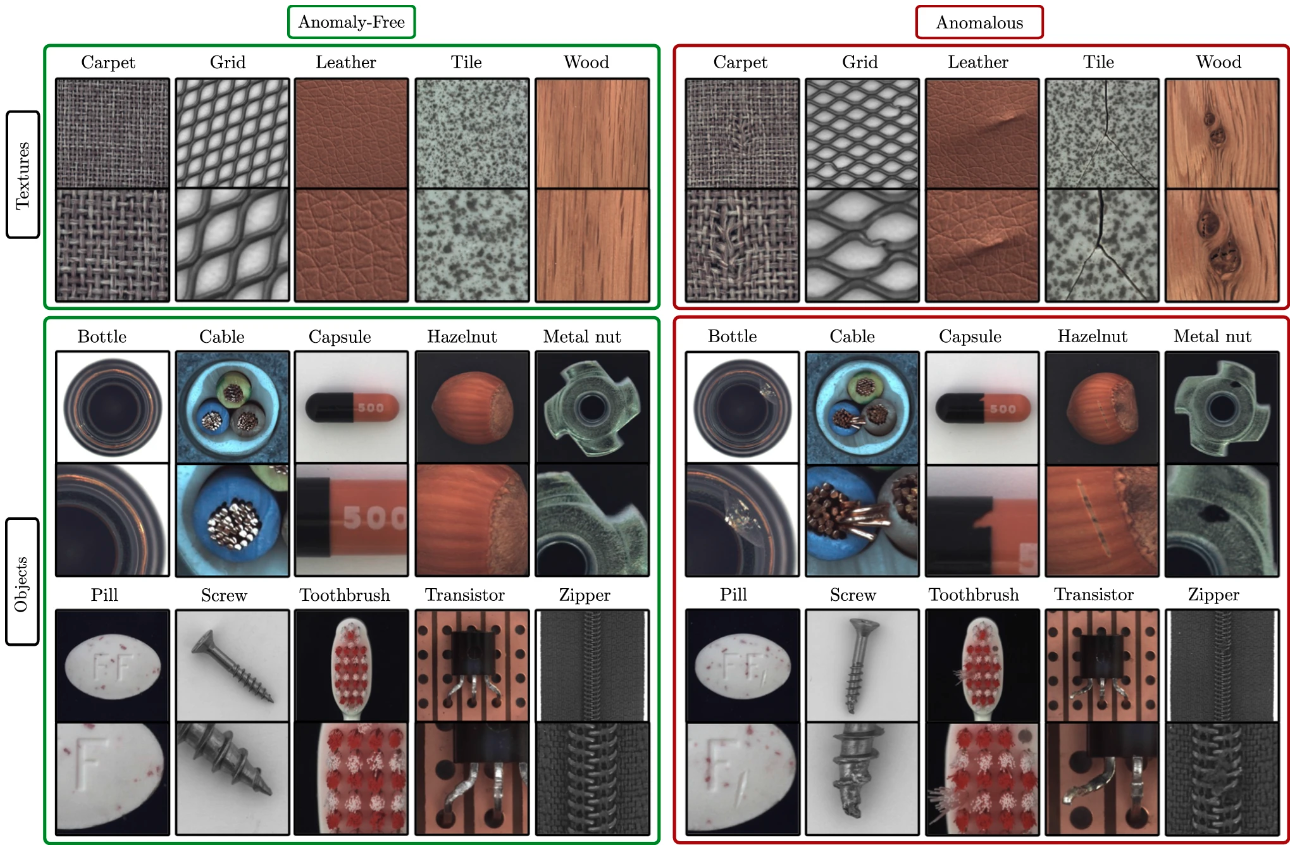
\includegraphics[width=0.95\textwidth]{bilder/mvtecad_examples.png}
  \caption{Beispiele für nominale und anomale Bilder aus dem MVTec AD Datensatz}
  \label{fig:mvtecad_examples}
\end{figure}


\section{Eigener Datensatz (Granulat)}\label{sec:EigenerDatensatz}
Details und Beispiele zu eigenem Datensatz.

\section{AUROC\cite{aurcoc}}\label{sec:AUROC}
In dieser Arbeit, genauso wie in beinahe allen anderen Arbeiten im Bereich der binären Anomalieerkennung, wird die \glqq Area Under the Receiver Operating Characteristic Curve\grqq{} (AUROC) als Leistungsmaß verwendet.\ 
Die AUROC ist ein Maß für die Fähigkeit eines binären Klassifikators, zwischen zwei Klassen zu unterscheiden. \
Nachfolgend wird schrittweise zum Begriff des AUROC hingeführt. \
\subsection{Logistische Regression}\label{subsec:LogistischeRegression}
%Die logistische Regression ist eine Methode zur binären Klassifizierung, bei der das Ziel darin besteht, ein binäres Ergebnis auf der Grundlage einer Reihe von Eingabemerkmalen vorherzusagen. \
%Bei der logistischen Regression gibt ein statistisches Modell einen Wahrscheinlichkeitswert zwischen 0 und 1 aus, der als die Wahrscheinlichkeit der positiven Klasse interpretiert werden kann. Um eine binäre Vorhersage \ 
%zu treffen, wird ein Schwellenwert auf den Wahrscheinlichkeitswert angewandt, so dass Werte oberhalb des Schwellenwerts als positiv und Werte unterhalb des Schwellenwerts als negativ eingestuft werden. \
Die logistische Regression ist eine Art verallgemeinertes lineares Modell, das üblicherweise für binäre Klassifizierungsprobleme verwendet wird. \ 
Bei der logistischen Regression besteht das Ziel darin, die Wahrscheinlichkeit eines binären Ergebnisses (z. B. nominal oder anomal) auf der Grundlage einer Reihe von Eingangsmerkmalen vorherzusagen. \ 
Das logistische Regressionsmodell verwendet eine logistische Funktion (\glqq Sigmoidfunktion\grqq{}), um die Eingabemerkmale auf die vorhergesagte Wahrscheinlichkeit abzubilden. \

Die logistische Funktion ist definiert als: \
$$ 
\sigma(z) = \frac{1}{1 + e^{-z}} 
$$

wobei $z$ eine lineare Kombination aus den Eingangsmerkmalen und ihren zugehörigen Gewichten ist: \

$$ 
z = \beta_0 + \beta_1 x_1 + \beta_2 x_2 + \cdots + \beta_p x_p 
$$

Dabei ist $\beta_0$ der Bias-Term und $\beta_1, \beta_2, \ldots, \beta_p$ sind die Koeffizienten für die Eingangsmerkmale $x_1, x_2, \ldots bzw. x_p$.

Das logistische Regressionsmodell wird trainiert, indem eine Verlustfunktion minimiert wird, die die Differenz zwischen den vorhergesagten Wahrscheinlichkeiten \ 
und den wahren binären Kennzeichnungen misst. Eine gängige Verlustfunktion für logistische Regression ist der binäre Kreuzentropie (\glq Cross-Entropy\grqq{}), die wie folgt definiert ist: \

$$ 
\mathcal{L}(\beta) = -\frac{1}{n} \sum_{i=1}^n y_i \log(\hat{y}_i) + (1 - y_i) \log(1 - \hat{y}_i)
$$

wobei $\beta$ die Modellparameter (d.h. den Achsenabschnitt und die Koeffizienten) darstellt, $n$ die Anzahl der Trainingsbeispiele, \ 
$y_i$ das wahre binäre Label für das $i$-te Beispiel und $\hat{y}_i$ die vorhergesagte Wahrscheinlichkeit für das $i$-te Beispiel ist. \

Das logistische Regressionsmodell kann mithilfe des Gradientenabstiegs trainiert werden, bei dem die Modellparameter iterativ in Richtung des negativen Gradienten der Verlustfunktion \ 
aktualisiert werden. Der Gradient der Verlustfunktion in Bezug auf die Modellparameter kann mithilfe der Kettenregel der Infinitesimalrechnung berechnet werden. \
\cite{bishop2006pattern} (Kapitel 4) \cite{intoStatLearn}
\subsection{Konfusionsmatrix}\label{subsec:Konfusionsmatrix}
Die Konfusionsmatrix ist eine Tabelle, die die Leistung eines binären Klassifikationsmodells zusammenfasst. Sie besteht aus vier Einträgen: wahr-positive (TP), falsch-positive (FP), wahr-negative (TN) und falsch-negative (FN). \ 
TP und TN stehen für die Anzahl der richtig klassifizierten positiven bzw. negativen Beispiele, während FP und FN für die Anzahl der falsch klassifizierten positiven bzw. negativen Beispiele stehen.
\begin{table}[h]
  \centering
  \begin{tabular}{|c|c|c|}
  \hline
   & \textbf{Tatsächlich Positive} & \textbf{Tatsächlich Negative} \\
  \hline
  \textbf{Prädizierte Positive} & Wahre Positive (TP) & Falsche Positive (FP) \\
  \hline
  \textbf{Prädizierte Negative} & Falsche Negative (FN) & Wahre Negative (TN) \\
  \hline
  \end{tabular}
  \caption{Konfusionsmatrix}
  \label{tab:Konfusionsmatrix}
\end{table}

Hier stehen die Zeilen für die vorhergesagten Kennzeichnungen und die Spalten für die wahren Kennzeichnungen. Die Einträge in der Diagonale stehen für die richtigen Vorhersagen, \ 
während die Einträge außerhalb der Diagonale die falschen Vorhersagen darstellen. \
Die \glqq True Positive Rate\grqq{}(TPR), die auch als Sensitivität oder Recall bezeichnet wird, ist definiert als TP / (TP + FN), d. h. der Anteil der positiven Beispiele, die richtig klassifiziert \ 
wurden. Die \glqq False Positive Rate\grqq{} (FPR) ist definiert als FP / (FP + TN), d. h. der Anteil der negativen Beispiele, die falsch klassifiziert werden. \
Die Konfusionsmatrix bietet eine Möglichkeit, die Leistung eines binären Klassifikationsmodells im Hinblick auf seine Fähigkeit, positive und negative Beispiele richtig zu klassifizieren, \ 
zu bewerten. Sie kann zur Berechnung verschiedener Leistungsmetriken verwendet werden, wie z. B. Genauigkeit, Präzision, Wiedererkennung, F1-Score und die Fläche unter der \glqq Receiver Operating Characteristic\grqq{} (ROC)-Kurve (AUC), \ 
die im nächsten Abschnitt erläutert wird.
\subsection{ROC-Kurve}\label{subsec:ROC-Kurve}
Die Receiver-Operating-Characteristic-Kurve (ROC-Kurve) ist eine grafische Darstellung der Leistung eines binären Klassifikationsmodells, wenn der Schwellenwert variiert wird.\ 
In der ROC-Kurve wird die Rate der richtig positiven Beispiele (TPR) \ 
gegen die Rate der falsch positiven Beispiele (FPR) für verschiedene Schwellenwerte aufgetragen. Die TPR ist der Anteil der positiven Beispiele, die richtig klassifiziert werden, \ 
während die FPR der Anteil der negativen Beispiele ist, die falsch klassifiziert werden. \\
Berechnet man die Fläche unter der ROC-Kurve erhält man das \textbf{\glqq Area Under the Curve\grqq{} (AUC)} Maß. Es ist eines der aussagekräftigsten Maße, die es für eine binäre Klassifikation \
wie die Anomalieerkennung gibt. Die AUC ist ein Wert zwischen $0$ und $1$, wobei $1$ für eine perfekte Klassifikation steht, $\num{0,5}$ für eine zufällige Klassifikation und $0$ für eine gänzlich falsche Klassifikation steht. \
Nachfolgend sind mögliche Ausbabeverteilungen einer logistischen Regression, markiert mit der tatsächlichen Klassenzugehörigkeit, skizziert. Diese Veranschaulichen den Zusammenhang zwischen der Ausgabe einer logistischen Regression, \
der ROC-Kurve und dem AUROC-Maß.
\newcommand{\thiswidth}{0.8\textwidth}
\begin{figure}[h]
  \centering
  \begin{subfigure}[b]{\thiswidth}
      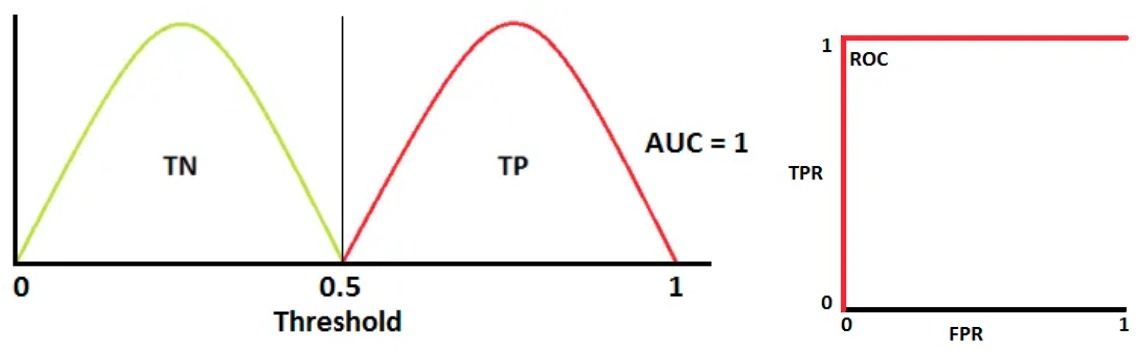
\includegraphics[width=\linewidth]{bilder/auc_1.png}
      \caption{$\mathbf{AUC = \num{100}\%}$: Die beiden Verteilungen der Klassen sind vollständig getrennt. Eine perfekte Klassifikation ist möglich.}
      \label{fig:subfig1}
  \end{subfigure}
  \hfill
  \begin{subfigure}[b]{\thiswidth}
      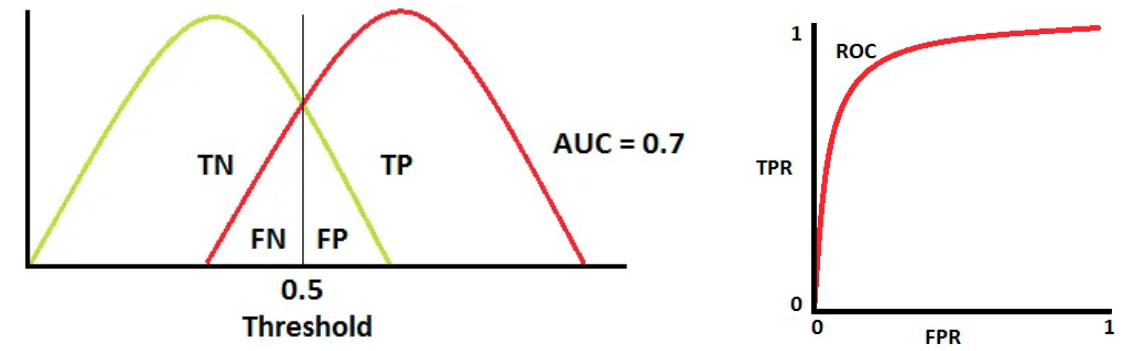
\includegraphics[width=\linewidth]{bilder/auc_07.png}
      \caption{$\mathbf{AUC = \num{70}\%}$: Eine Überlappung der Verteilungen lässt mit keinem Schwellwert eine fehlerfreie Klassifikation zu. Ein Großteil der Beispiele kann aber richtig klassifiziert werden.}
      \label{fig:subfig2}
  \end{subfigure}
  
  \begin{subfigure}[b]{\thiswidth}
      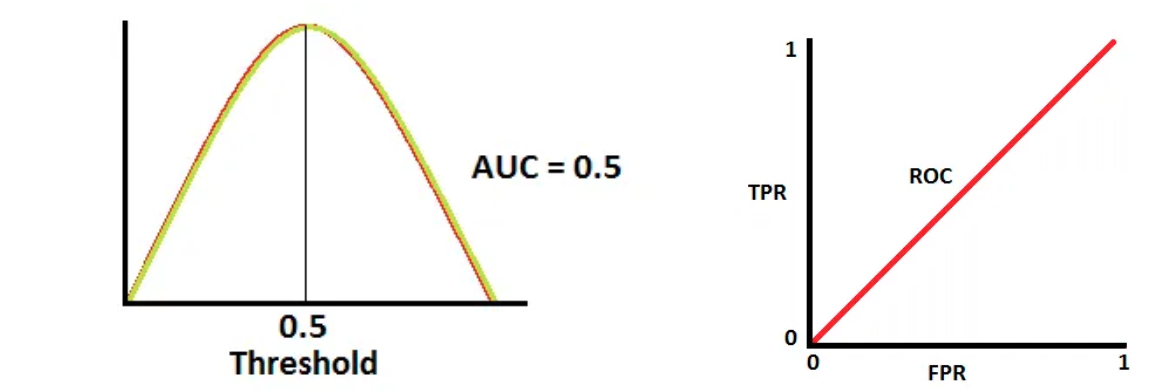
\includegraphics[width=\linewidth]{bilder/auc_05.png}
      \caption{$\mathbf{AUC = \num{50}\%}$: Die Verteilungen der Klassen überlappen sich vollständig. Eine sinnvolle Klassifikation ist somit nicht möglich. Eine Zuordnung würde zufällig geschehen.}
      \label{fig:subfig3}
  \end{subfigure}
  \hfill
  \begin{subfigure}[b]{\thiswidth}
      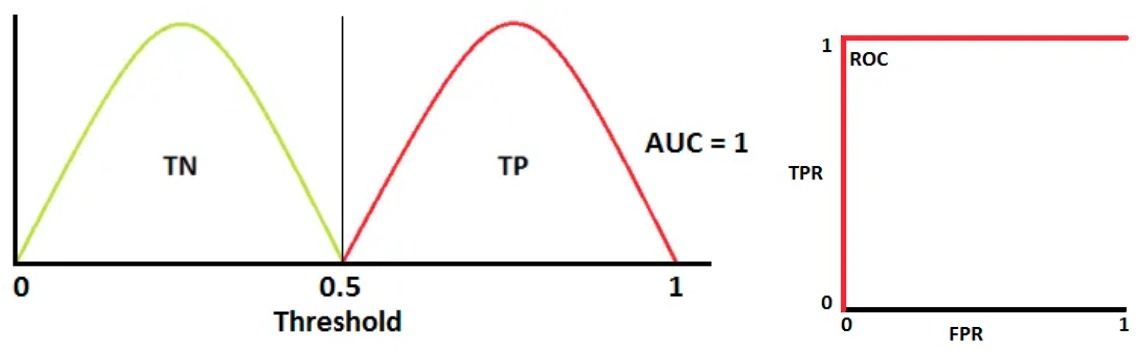
\includegraphics[width=\linewidth]{bilder/auc_1.png}
      \caption{$\mathbf{AUC = \num{0}\%}$: Dieser Spezialfall lässt keine korrekte Klassifikation zu, obwohl die Klassen eindeutig getrennt sind. Dies liegt daran, dass die Verteilung der positiven Klasse vollständig links von der Verteilung der negativen Klasse liegt. Durch eine geeignete Abbildung kann dieses Problem gelöst werden.}
      \label{fig:subfig4}
  \end{subfigure}
  \caption{Veranschaulichung verschiedener Verteilungen positiver und negativer Klassen und den dazugehörenden ROC-Kurven und AUC-Werten.}
  \label{fig:main}
\end{figure}
\newpage
\section{Residuale Netzwerke}\label{sec:ResidualNetworks}
In diesem Abschnitt werden die Grundlagen von Residual Networks (textbf{\glqq ResNets\grqq{}}) erläutert. \
Diese spielen für die Merkmalsextraktoren (\glqq Feature Extractors\grqq{}) in den im Haupteil der Arbeit (TODO --> Link) eine wichtige Rolle. \
Der Schwerpunkt hierbei liegt auf der grundlegenden Idee, der Rolle, die ResNets historisch in der Entwicklung von Deep Learning gespielt haben und \
vor allem den Aspekten, die für die Anwendung in dieser Arbeit relevant sind. \ 
Für detailierte Informationen zu ResNets wird auf das Paper von Kaiming He et al. \cite{resnet} und die zahlreichen Erläuterungen in der Literatur verwiesen. \
\subsection{Hintergrund \& Idee hinter \glqq ResNets\grqq{}}\label{subsec:ResNetsBackgroundAndIdea}
Tiefe neuronale Netze (Deep Neural Networks, DNNs) eignen sich hervorragend für das Lernen hierarchischer Darstellungen aus Daten,\
aber sie stehen vor Herausforderungen, wenn sie \glqq tiefer\grqq{} werden.\glqq Tiefe\grqq{} bezeichnet in diesem Zusammenhang \ 
die Anzahl an Schichten, die sequentiell durchlaufen werden, um das Endergebnis bzw. die Ausgabe zu erhalten. \
Tiefere Netze können komplexere Merkmale in Daten erfassen, was für Aufgaben wie die Bildklassifizierung, bei der Objekte und Muster komplizierte Details aufweisen können, entscheidend ist.\
Einer der großen Herausforderungen bei tiefen Netzen ist das Problem der \glqq verschwindenden Gradienten\grqq{} (\textit{engl.} \textbf{Vanishing Gradients}). \
Diese Gradienten sind entscheidend für das Training eines Neuronalen Netzes, insofern, als dass das Optimierungsverfahren des Gradientenabstiegs die Grundlage auch moderner Optimierer wie \glqq Adam\grqq{} (TODO --> Ref) ist. \ 
Dieses Problem lässt sich anschaulich dadurch erklären, dass frühe Gradienten, was sich leicht mithilfe der Kettenregel zeigen lässt, \ 
eine Multiplikation von allen nachfolgenden (im Sinne der Infernenzrichtung - \glqq forward pass\grqq{}) Gradienten darstellt. \
Betrachtet man nun ein sehr tiefes Netz, das heißt, viele Gradienten, die miteinander multipliziert werden und den wahrscheinliche Fall von Gradienten, die kleiner als $1$ sind, so wird schnell klar, dass frühe Schichten einen sehr kleinen Gradienten haben können. \
Dies macht es schwierig, die Gewichte der frühen Schichten zu aktualisieren, was den Lernprozess behindert. Dabei ist es vor allem die Tiefe, die Neuronalen Netzen das Generalisieren von komplexen Zusammenhängen ermöglicht (\glqq Deep Learning \grqq{})\\
Residuale Netze, allgemein bekannt als ResNets und im Folgenden auch so bezeichnet, wurden von Kaiming He et al. (TODO --> Ref) in ihrem Paper von 2015 vorgestellt und bieten eine einfache und dennoch effektive Methode an, wie dieses Problem angegangen werden kann. \
Die Grundidee besteht darin, Verknüpfungen zwischen den Schichten einzuführen, die es dem Netz ermöglichen, eine oder mehrere Schichten zu \glqq überspringen\grqq{}. \ 
Anstatt die gewünschte Abbildung also direkt zu lernen, lernen ResNets die residuale Abbildung, was der Differenz zwischen Ein- und Ausgabe entspricht. Die Eingabe wird über sogenannte \
\glqq Shortcut (Skip) Connections\grqq{}, also einfach die Identitätsabbildung, vom Eingang zur residualen Ausgabe weitergeleitet, um dann durch Summation wieder miteinander verknüpft zu werden. \
Das Problem der verschwindenden Gradienten wird dadurch entschärft, dass die Gradienten direkt in frühere Schichten zurückfließen können. 
Anschaulich lässt sich das durch die Tatsache erklären, dass die Identitätsabbildung einen konstanten Gradienten von $1$ besitzt. Weil sich die Summenbildung \
am Ausgang eines nachfolgend noch im Detail besprochenen Residual-Blocks auch bei der Gradientenbildung als Summation widerspiegelt, ist der Gradient einer jeden Schicht nicht mehr das Produkt, sondern vielmehr die Summe aller nachfolgenden Gradienten. (Optional TODO: Formel) 
Das zugrundeliegende Paper ist eines der meistzitierten Paper im Bereich des Deep Learning und hat die Entwicklung von Deep Learning maßgeblich beeinflusst. \
\subsection{Residual Block \& Architektur}\label{subsec:ResidualBlocks}
Der Grundbaustein eines ResNet ist der Residualblock. Er besteht aus zwei Hauptpfaden: dem Identitätspfad (der Abkürzungsverbindung) und dem Residualpfad (dem Hauptfaltungspfad).\ 
Mathematisch wird die Ausgabe eines Residualblocks wie folgt berechnet:
\[
\text{Output} = F(\text{Input}) + \text{Input}
\]
wo $F$ die Residualabbildung ist, die durch die Hauptfaltungsschichten gelernt wird.\  
%The shortcut connection allows the gradients to flow directly back to earlier layers without vanishing, making it easier for the network to learn.
Nachfolgende Abbildung zeigt eine vereinfachte Darstellung eines \glqq Building Blocks\grqq{} bzw. Residual Block. \
\begin{figure}[H]
  \centering
  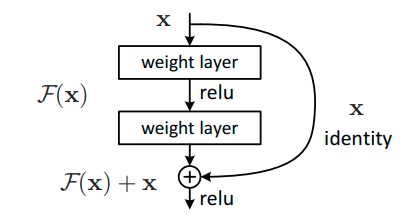
\includegraphics[width=0.5\textwidth]{bilder/residual_block.png}
  \caption{Residual Block (TODO --> Ref)}
  \label{fig:ResidualBlock}
\end{figure}
Ein ResNet besteht aus mehreren Residualblöcken, die sequentiell durchlaufen werden. Es ist also eine \glqq Feed-Forward\grqq{}-Architektur, weil die Daten zur Inferenz \ 
nur in eine Richtung durch das Netz fließen. Durch das \glqq Stapeln \grqq{} können dann sehr tiefe Netze erstellt werden, die sich dennoch aufgrund der oben beschriebenen
Eigenschaften gut optimieren bzw. trainieren lassen. \\
Es existieren zahlreiche verschiedene Varianten von ResNets, die sich in der Art und Anzahl ihrer Residual Blöcke unterscheiden. \
Nachfolgende Tabelle gibt einen Überblick über die drei, in dieser Arbeit vor allem verwendeten Varianten: ResNet18, ResNet34 und WideResNet50 \

\begin{table}[h]
  \centering
  \begin{tabular}{|c|c|c|c|c|}
  \hline
  \textbf{Netzwerk} & \textbf{Tiefe} & \textbf{\# Parameter} & \textbf{Top-1 Fehlerrate\tablefootnote{in ILSVRC (TODO --> Ref)}} & \textbf{Inferenz auf RBP4\tablefootnote{Raspberry Pi 4B 8GB. Betrachtet wurde die Laufzeit von einem Bild der Auflösung 224x224 und 3 (Farb-)Kanälen}} \\ \hline
  ResNet18         & \makecell{$18$}             & \makecell{$\num{11,7e6}$}                        & \makecell{$\num{30.24}$\%}                   & \makecell{$0,82\si{\second}$}\\ \hline
  ResNet34         & \makecell{$34$}             & \makecell{$\num{21,8e6}$}                       & \makecell{$\num{26.70}$\%}                   & \makecell{$1,45\si{\second}$}\\ \hline
  WideResNet50     & \makecell{$50$}             & \makecell{$\num{68,9e6}$}                        & \makecell{$\num{22.53}$\%}                   & \makecell{$3,00\si{\second}$}\\ \hline
  \end{tabular}
  \caption{Vergleich verschiedener ResNet Varianten (TODO --> Ref)}
  \label{tab:resnet-comparison}
\end{table}
Zu erkennen ist eindeutig, dass die Anzahl der Parameter und die Inferenzzeit mit der Tiefe des Netzes steigt. \
Gleichzeitig lässt sich aber auch eine Verbesserung der Top-1 Fehlerrate erkennen, je tiefer bzw. mächtiger das Netz ist. \\
Einer der Hauptvorteile von ResNets ist die Fähigkeit, Merkmale pyramidenförmig durch das Netz zu verbreiten. Das bedeutet, dass das Netz Merkmale auf verschiedenen \ 
Abstraktionsebenen erfassen kann, von Low-Level-Merkmalen wie Kanten und Ecken bis zu High-Level-Merkmalen wie Objektteilen und semantischen Konzepten. \
Mit zunehmender Tiefe wird also die Auflösung der \glqq Feature Maps\grqq{} (TODO --> Ref) reduziert, während die Anzahl der Kanäle und die Komplexität der zugrundeliegenden Merkmale zunimmt. \
Dargestellt ist das in folgender Abbildung:
\begin{figure}[H]
  \centering
  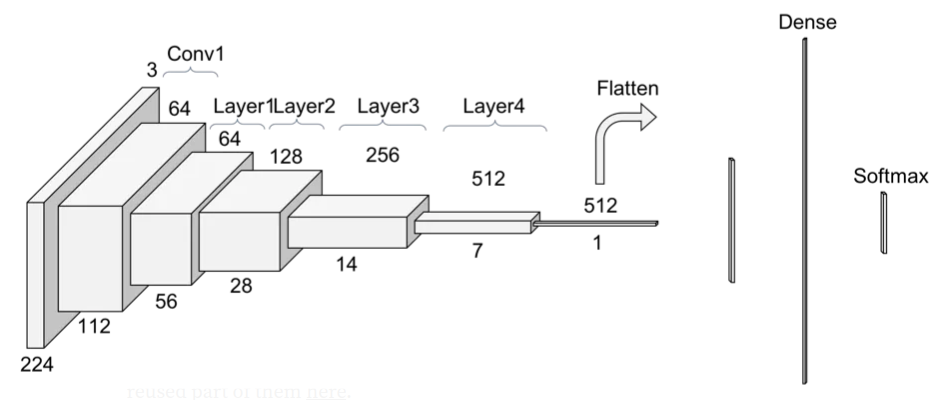
\includegraphics[width=0.8\textwidth]{bilder/resnet_pyramid.png}
  \caption{Pyramidale Merkmalsverteilung in ResNets (TODO --> Ref)}
  \label{fig:ResNetPyramid}
\end{figure}
Die Quader in oben stehendem Netz stehen symbolhaft für die Auflösung der Feature Maps. \
Während die oben stehenden Zahlen die Anzahl der Kanäle repräsentieren, stehen die unten aufgeführten Zahlen für die räumliche Auflösung. Letztere hängt \ 
proportional von der Auflösung des Eingangsbildes ab und gilt für alle drei Modelle. Die Anzahl an Kanälen ist konstant für alle Auflösungen und für ResNet18 und ResNet34. \
Für das WideResNet50 gilt im Wensentlichen der gleiche Aufbau, allerdings sind die Kanäle \glqq geweit\grqq{} gegenüber den anderen beiden Architekturen, was \
sich an der Vervierfachung der Anzahl an Kanäle durch Verwendung eines komplexeren Residual Blocks (\glqq Bottleneck\grqq{}\cite{wideresnet})zeigt. 
ResNet18 und ResNet34 unterscheiden sich ausschließlich in der Anzahl der Residual Blöcke bzw. der Tiefe des Netzes. \\
Alle der drei hier vorgestellten Architekturen lassen sich in fünf Faltungsschichten (\glqq Conv1\grqq{}, \glqq Layer1\grqq{}, \glqq Layer2\grqq{}, \glqq Layer3\grqq{}, \glqq Layer4\grqq{}) unterteilen. \
Dem schließt sich eine \glqq Average Pooling\grqq{}-Schicht an, die die Auflösung der Feature Maps auf 1 reduizert (\glqq Flatten\grqq{}). Dieser 1D-Vektor wird \
schließlich durch eine \glqq Fully Connected\grqq{}-Schicht (\glqq Dense\grqq{}) auf die Anzahl der Klassen (1000) abgebildet. Schließlich wird durch eine \glqq Softmax\grqq{}-Aktivierungsfunktion \
Pseodo-Wahrscheinlichkeiten erzeugt, die den Axiomen von Kolmogorov entsprechen und somit als Auftrittswahrscheinlichkeiten interpretiert werden können.\\
In dieser Arbeit werden die ResNets als Feature-Extraktoren verwendet, weshalb die letzten beiden Schichten, also \glqq Flatten\grqq{} und \glqq Dense\grqq{} nicht verwendet werden. \ 
Die Begriffe \glqq Layer1 - Layer4\grqq{} werden im Folgenden in dem hier beschriebenen Kontext verwendet. \\ 
\subsection{ResNets as Feature Extractor für Unüberwachte Lernverfahren}\label{subsec:ResNetsAsFeatureExtractor}
Zusätzlich zu ihrem Erfolg bei der überwachten Bildklassifizierung haben ResNets Anwendungen als leistungsstarke Merkmalsextraktoren bei Unüberwachten Klassifizierungsaufgaben \ 
wie der Anomalieerkennung gefunden. In unüberwachten Szenarien wie der Anomalieerkennung stehen oft keine markierten (gelabelten) Daten zur Verfügung, wie bereits in \ref{sec:UnueberwachteAnomaliedetektion} beschrieben, um ein Modell explizit bzw. überwacht zu trainieren. \ 
Stattdessen verlässt man sich auf das Lernen von Darstellungen normaler Daten und identifiziert dann Abweichungen als Anomalien. ResNets können mit ihrer Fähigkeit, umfangreiche und hierarchische Merkmale \ 
zu erfassen, dazu verwendet werden, sinnvolle Merkmale aus den Daten zu extrahieren. Es kann mithilfe dieser Netze eine kompaktere und aussagekräftigere Darstellung der Daten erzeugt werden, die die Grundlage sind, \
um auch komplexere Anomalien zu erkennen. Allerdings ist festzuhalten, dass die extrahierten Feature in keiner Weise optimiert sind, um Anomalieklassifikationen zu ermöglichen, sondern um auf dem ImageNet-Datensatz \
Bilder richtig einzuordnen. Vor allem in späteren Schichten ist also zu erwarten, dass die Merkmale einene \glqq Bias \grqq{} hin zu ImageNet aufweisen, der sich negativ auf die Anomalieklassifikation auswirken kann.\cite{patchcore} \ 
Hierzu werden die Gewichte offizieller Implementierungen von ResNets verwendet, womit das eigentliche Vortraining \ 
entfällt und Reproduzierbarkeit, Konsistenz und Vergleichbarkeit der Ergebnisse gewährleistet wird. \\
Alle hier vorgestellten Methoden verwenden ResNets als Feature-Extraktoren, wenn auch im Ansatz\glqq EffientAD\grqq{} (\ref{ch:EfficientAD}) nicht während der Inferenz. \
Gezeigt, dass eine solche Feature Extraktion im Kontext der Unüberwachten Anomalieerkennung sinnvoll ist, wurde erstmals in der Veröffentlichung\glqq Deep Nearest Neighbor Anomly Detection\grqq{} von Bergman et al.\cite{DN2} mit der Methode \glqq DN2\grqq{} im Februar 2020. \
Im nachfolgenden Abschnitt wird die darauf aufbauende Methode \glqq SPADE\grqq{}, vom gleichen Team entwickelt, vorgestellt. \
% \section{Autoencoder}\label{sec:Autoencoder}
% Hier kommt dann eine relativ generische Erläuterung von Autoencodern. \
% Gefolgt von Autoencoder für Anomaliedetektion. \
\section{SPADE}\label{sec:SPADE}
Die Methode \textbf{SPADE} ist ein wichtiger Meilenstein in der Unüberwachten Anomalieerkennung.\
Zahlreiche erfolgreiche Methoden bauen auf SPADE auf und übernehmen wichtige Elemente und Konzepte.\
Das Paper wurde am 5. Mai 2020 von Niv Cohen und Yedid Hoshen von der Hebräischen Universität von Jerusalem veröffentlicht.\
Im Folgenden wird SPADE vorgestellt.\
\subsection{Funktionsweise}\label{subsec:SPADEFunktionsweise}
\subsubsection*{Feature Extraktion}
Wie bereits in \ref{subsec:ResNetsAsFeatureExtractor} beschrieben, werden ResNets erfolgreich als Feature-Extraktoren verwendet.\
Der Name \glqq SPADE\grqq{} steht hierbei für \glqq Semantic Pyramid Anomaly Detection\grqq{}. Betrachtet man \ref{fig:ResNetPyramid} wird klar warum von einer \glqq Pyramide\grqq{} gesprochen werden kann:\
Es werden die Feature Maps der einzelnen Schichten, konkret der Schichten \glqq Layer1, Layer2 und Layer3\grqq{} als Feature unverändert verwendet.\
Dabei wird auf einen Einbettungsprozess, wie bei anderen Methoden üblich, verzichtet.\ Durch die mit der Tiefe des Netzes abnehmende Auflösung der Feature Maps, \
entsteht so eine \glqq Pyramidale\grqq{} Struktur, die eben die Grundlage für die Namensgebung ist.\
Zusätzlich wird der 1D-Vektor, der durch die \glqq Flatten\grqq{}-Schicht erzeugt wird, als Feature verwendet, um instanzweise, also für jedes Bild als Ganzes, zu entscheiden, ob eine \
Anomalie vorliegt, wie im nächsten Abschnitt beschrieben.\
Bezeichnen wir das ResNet als Feature-Extraktor mit $F$, so lassen sich die Feature $f_{i}$ eines gegebenen Bildes $x_{i}$ wie folgt beschreiben:
$$f_{i} = F(x_{i})$$
In der Trainings- bzw. Initialisierungsphase werden die Feature $f_{i}$ aller Trainingsbilder $x_{i}$, welche alle nominal sind, extrahiert und gespeichert.\
Diese Menge wird im Folgenden mit $F_{train}$ bezeichnet.\
\subsubsection*{Instanzklassifizierung}
Die Instanzklassifizierung ist der zweite Schritt von SPADE. Es wird dabei für jedes Bild $y_{i}$ aus der Menge an Testbilder $Y$ entschieden, ob es sich um eine Anomalie handelt oder nicht.\
Dies geschieht ausschließlich anhand des 1D-Vektors, der durch die \glqq Flatten\grqq{}-Schicht erzeugt wird.\
Hierzu wird für ein gegebenes Testbild $y_{i}$, die $K$ nächsten Nachbarn in $F_{train}$ gesucht. Diese Menge an $K$ Vektoren wird fortan als $N_{k}(f_{y})$ bezeichent. \
Es wird eine Distanz auf die folgende Art und Weise bestimmt:
$$
d(y_{i}) = \frac{1}{K} \sum_{f\in N_{k}(f_{y_{i}})} \left|\left| f - f_{y_{i}} \right|\right|^{2}
$$
Die Distanz $d(y_{i})$ wird dann mit einem Schwellenwert $\tau$ verglichen. Ist die Distanz kleiner als der Schwellenwert, so wird das Bild als nominal klassifiziert, ansonsten als Anomalie.\
\subsubsection*{Segmentierung}
Nachdem eine Instanzklassifiziergung ergeben hat, dass es sich um ein anomales Bild handelt, besteht die nächste Aufgabe darin, die Anomalie oder mehrere Anomalien auf dem Bild zu lokalisieren.\
Dieser Schritt wird übersprungen, wenn das Bild als nominal klassifiziert wurde.\\
Die naive Methode, die Anomalie zu lokalisieren, wäre es, die Differenz zwischen dem anomalen Bild und dem ausgerichtete Bild des nächsten Nachbarn zu berechnen. Dort, wo die Differenz am größten ist, \
wird die Anomalie vermutet. Allerdings hat diese Methode einige Schwachstellen. Zum einen kann die Ausrichtung des nächsten Nachbarn so, dass das zu untersuchende Objekt im Bild an der gleichen Stelle ist, \
fehlschlagen. Insbesondere. Auch kann insbesondere bei eienem kleinen Datensatz und Objekten, die komplexe Variationen aufweisen möglicherweise kein passender Nachbar gefunden werden, was zu falsch positiven (anomalen) \
Klassifizierungen führen kann. Außerdem könnte die Berechnung der Differenz sehr empfindlich auf die verwendete Berechnungsmethode sein.(TODO... Vllt einfach weg lassen?)\\ 
Um diese Probleme zu überwinden, wird eine Übereinstimmungsmethode präsentiert, die mit vielen \glqq Bildern\grqq{} arbeitet (\glqq multi-image correspondence method\grqq{}). Diese Bilder entsprechen den Feature Maps der Schichten Layer1, Layer2 und Layer3, \
also gewissermaßen den Quader in \ref{fig:ResNetPyramid}.\\
Nun gilt es zu jeder Pixelposition $p\in P$ die korresponierenden Feature $F(x_{i}, p | p\in P)$ zu bestimmen. Auf jedes Bild aus dem Trainingsdatensatz $x_{i}$ \ 
angewandt und ergibt sich dann die \glqq Gallerie\grqq{} zu $G = \{ {F(x_{1}, p | p\in P)}\cup {F(x_{2},p|p\in P)} .. \cup {F(x_{K},p|p\in P)} \}$.\\
Der Anomaliegrad eines Pixels $p$ ist dann gegeben durch die durchschnittliche Distanz zwischen dem Feature $F(y_{i},p)$ des anomalen Bildes $y_{i}$ und \ 
den $\kappa$ nächsten Featuren aus der Gallerie $G$. Es ergibt sich also für einen Pixel $p$ im Testbild $y_{i}$ folgende Formel: \
$$
d(y_{i},p) = \frac{1}{\kappa} \sum_{f\in N_{\kappa}(F(y_{i},p))} \left|\left| f - F(y_{i},p) \right|\right|^{2}
$$
Für einen gegebenen Schwellwert $\theta$ wird ein Pixel $p$ als anomales Pixel klassifiziert, wenn $d(y_{i},p) > \theta$ gilt.
Dies ist dann der Fall, wenn wir kein nominales Feature in $G$ finden können, welches dem Feature $F(y_{i},p)$ ausreichend ähnlich ist.\\
Dadurch, dass die Gallerie $G$ die Positionsinformation $p$ marginalisiert, wird die Segmentierung robust gegenüber der Ausrichtung. Anschaulich gesprochen, wird \
also in jedem Bild an allen Positionen nach ähnlichen Features gesucht.
\subsection{Ergebnisse und Diskussion}\label{subsec:SPADEResults}
Wie bereits erwähnt, markiert diese Arbeit einen wichtigen Entwicklungsschritt in der Forschung zur Unüberwachten Anomalieerkennung. \
Folgende Aspekte sollten in diesem Zusammenhang hervorgehoben werden:
\begin{itemize}
  \item SPADE ist die erste ganzheitliche Methode, die auf ImageNet vortrainierte ResNets als Feature-Extraktoren verwendet. Dieser Ansatz hat sich als sehr erfolgreich erwiesen und wird von zahlreichen Methoden übernommen. \
  \item Das Zusammenfassen aller extrahierten Features aus den Testbildern zu einer Menge $G$ löst das Problem der Ausrichtung und ermöglicht eine robuste Segmentierung. Auch diese Idee wird uns bei PatchCore (\ref{ch:PatchCore}) wiederbegegnen.\
  \item Das Bestimmen des Anomaliegrades mithilfe einer kNN-Suche ist ein einfacher und effektiver Ansatz, der sich auch in modifizierter Form in vielen anderen Methoden wiederfindet.\
\end{itemize}
Insbesondere in der pixelweisen Klassifikation von Anomalien hat sich SPADE als geeignet erwiesen. Auch in der Instanzklassifiziergung erreicht diese Methode auf dem damals \
noch jungen Datensatz MVTecAD gute, zum Zeitpunkt der Veröffentlichung der Methode, sogar das beste Ergebnisse.\\
Für das Ziel dieser Arbeit, welche den Fokus auf die Instanzklassifiziergung und die Laufzeitoptimierung legt, ist SPADE allerdings eher ungeeignet. \
Zum Einen sind \num{85,5}\% erreichte Bildklassifizierungsgenauigkeit auf MVTecAD für die Instanzklassifizierung nicht mit neueren, zum Teil aber auf SPADE aufbauenden Methoden, konkurrenzfähig. \
Zum Anderen ist die notwendige kNN Suche, die für jedes Testbild durchgeführt werden muss, sehr rechenintensiv. Dieser Rechenaufwand skaliert linear mit der Anzahl an Bildern im Trainingsdatensatz und mit der Anzahl der Pixel pro Bild.\
Kann man auf eine Segmentierung verzichten, verkleinert sich der Rechenaufwand zwar deutlich, es muss aber dennoch eine kNN-Suche über alle Trainingsbilder für jedes Testbild durchgeführt werden, wodurch die Laufzeit wiederum von der Größe des Trainingsdatensatz abhängt, \ 
auch wenn die Auflösung der Bilder keinen Einfluss mehr hat. \
Den Anstoß und die Impulse, die durch diese Veröffentlichung gesetzt wurden, sind jedoch nicht zu unterschätzen. \

\section{PaDiM}\label{sec:PaDiM}
Die Methode \textbf{PaDiM} wurde am 17. November 2020 von Defard et al. (Universität Paris-Saclay) veröffentlicht.\
Es werden einige Aspekte von SPADE übernommen, vor allem aber Schwächen der Methode erfolgreich addressiert. Einer der wesentlichen Unterschiede zwischen PaDiM und SPADE ist, die Weise auf die der Anomaliescore bestimmt wird. \ 
PaDiM markierte damit die beste Instanzklassifizierungsgenauigkeit auf dem Datensatz MVTecAD zum Zeitpunkt der Veröffentlichung und hielt dies bis zum Erscheinen der Methode \glqq PatchCore\grqq{}.
Nachfolgend wird der Ansatz von PaDiM vorgestellt und diskutiert.\
\subsection{Funktionsweise}\label{subsec:PaDiMFunktionsweise}
\begin{figure}[H]
  \centering
  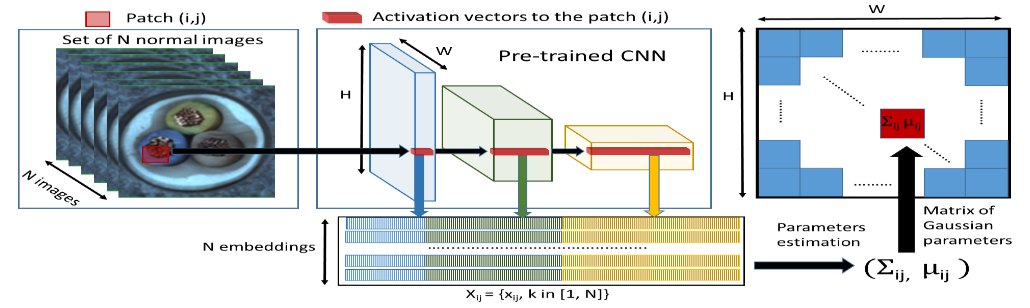
\includegraphics[width=0.8\textwidth]{bilder/padim.png}
  \caption{PaDiM: Funktionsweise (TODO --> Ref)}
  \label{fig:PaDiMOverview}
\end{figure}
% In \ref{fig:PaDiMOverview} ist die Funktionsweise von PaDiM dargestellt. \
PaDiM kann in drei Schritte unterteilt werden: \
\begin{enumerate}
  \item Feature Extraktion und Einbettungsprozess mithilfe eines vortrainierten ResNets
  \item Bestimmen der Gaußverteilungen durch Schätzen der Parameter $\mu$ und $\Sigma$ für jede Position im Bild
  \item Bestimmen des Anomaliegrades durch die Mahalanobis-Distanz
\end{enumerate}
\ref{fig:PaDiMOverview} veranschaulicht den Prozess exklusive der Inferenz. \
\subsubsection*{Feature Extraktion und Einbettungsprozess}
Der Prozess des Erzeugens von Featuren ist bei PaDiM sehr ähnlich zu dem von SPADE: \
Auch hier werden Feature Maps unterschiedlicher Auflösung und Abstraktionsebene zu einem Featurevektor zusammengefasst, der mit einer Position bzw. einem Pixel des Eingangsbildes korresponiert. \
Die Feature Map, welche die höchste Auflösung besitzt, also die Feature Map der ersten zur Feature Extraktion ausgewählten Schicht, definiert die Auflösung der Anomaliesegmentierung. \
Nehmen wir an diese Feature Map habe eine Auflösung von $W\times H$, so korresponiert also zu jeder Position $(i,j)\in [1,W]\times[1,H]$ ein Featurevektor $x_{ij}$ (\glqq Patch Embedding Vektor\grqq{}). \\
\subsubsection{Bestimmen der Gaußverteilungen}
PaDiM modelliert für jede Position eine multivariate Normalverteilung, die durch die Featurevektoren aller Trainingsbilder an dieser Position definiert wird. \\
Zunächst wird hierzu die Menge an Patch Embedding Vektoren für eine Position $(i,j)$ aus dem gesamten Trainingsdatensatz gebildet. Diese Menge \
$X_{ij} = \{ {x_{ij}^{k} | k\in [1,N]} \}$ aus den $N$ nominalen Bildern im Trainingsdatensatz wird dann benutzt, um die Normalverteilung für die Position $(i,j)$ zu bestimmen. \
Es wird also angenommen, $X_{ij}$ würde von der multivariaten Gaußverteilungen $N(\mu_{ij}, \Sigma_{ij})$ erzeugt werden. \
Die Parameter $\mu_{ij}$ und $\Sigma_{ij}$ werden dann wie folgt geschätzt: \
$$
\mu_{ij} = \frac{1}{N} \sum_{k=1}^{N} x_{ij}^{k}
$$
$$
\Sigma_{ij} = \frac{1}{N-1} \sum_{k=1}^{N} (x_{ij}^{k} - \mu_{ij})(x_{ij}^{k} - \mu_{ij})^{T} + \epsilon I
$$
wobei der Regularisierungsterm $\epsilon I$ hinzugefügt wird, um die Invertierbarkeit bzw. den vollen Rang der Kovarianzmatrix $\Sigma_{ij}$ zu gewährleisten. \
Schließlich wird die multivariate Gaußverteilung $N(\mu_{ij}, \Sigma_{ij})$ für jede Position $(i,j)$ im Bild definiert.\
\subsubsection{Bestimmen des Anomaliegrades}
Um den Anomaliegrad zu bestimmen, wird die Mahalanobis-Distanz herangezogen.%\cite{mahalanobis1936generalized} \
Die Mahalanobis-Distanz ist eine Verallgemeinerung der euklidischen Distanz, die die Korrelation zwischen den Dimensionen der Daten berücksichtigt. \
In diesem Fall lässt sich die Mahalanobis-Distanz für die Position $(i,j)$ und einem aus einem Testbild extrahierten Patch Embedding Vektor $y_{ij}$ wie folgt berechnen: \
$$
M(y_{ij}) = \sqrt{(y_{ij} - \mu_{ij})^{T} \Sigma_{ij}^{-1} (y_{ij} - \mu_{ij})}
$$
Damit kann dann eine Anomaliekarte $M$ für ein Testbild $y$ erzeugt werden:
$$
M = (M(y_{ij}))_{1<=i<=W, 1<=j<=H}
$$
Hierbei deuten hohe Werte auf eine Anomalie hin, während niedringe Werte auf einen nominalen Bildbereich hinweisen. \
Durch Maximalwerbildung über die Anomaliekarte $M$ kann dann ein Anomaliegrad $s$ für ein Testbild $y$ bestimmt werden: \
$$
s(y) = \max_{1<=i<=W, 1<=j<=H} M(y_{ij})
$$
\subsection{Ergebnisse und Diskussion}\label{subsec:PaDiMResults}
Wie bereits zu Beginn dieses Kapitels erwähnt, erreicht PaDiM zum Zeitpunkt der Veröffentlichung die beste Instanzklassifizierungsgenauigkeit auf dem Datensatz MVTecAD mit \num{97,5}\%. 
Auch die Segmentierungsergebnisse sind mit \num{97,9}\% zum Veröffentlichungszeitpunkt State-of-the-Art. \\
Ein spannender Aspekt, der in diesem Veröffentlichung untersucht wird, ist das Reduzieren der Anzahl an Kanälen bzw. die Reduzierung der Dimensionalität der Featurevektoren: \\
Es wird gezeigt, dass im Falle eines ResNet18 als Backbone die Dimensionalität von ursprünglich \num{448} auf \num{200} oder sogar \num{100} reduziert werden kann, ohne \
dass die Klassifizierungsgenauigkeit signifikant sinkt. Dabei wurden die zu entfernenden Dimensionen zufällig ausgewählt und die Ergenisse über mehrere Durchläufe gemittelt. \
Im Falle aller \num{448} Dimensionen wird eine Genauigkeit von \num{97,1}\% erreicht, während bei \num{200} Dimensionen eine Genauigkeit von \ 
\num{97,0}\% und bei \num{100} Dimensionen eine Genauigkeit von \num{96,7}\% erreicht wird. \\
Dies ist vor allem deshalb eine sehr relevante Erkenntnis, da die Reduzierung der Dimensionalität einen ganz erhebliche Einfluss auf die Berechnungsgeschwindigkeit der Mahalanobis-Distanz hat. \
Die Komplexität in der Landau-Notation für die Berechnung der Mahalanobis-Distanz zwischen zwei Vektoren der Länge $d$ ist $\mathcal{O}(d^{3})$\cite{bishop2006pattern}, \ 
wobei $d$ die Dimensionalität der Featurevektoren ist, in diesem Beispiel also \num{448}, \num{200} bzw. \num{100}. \
Dass der Einbruch der Genauigkeit bei einer Reduzierung der Dimensionalität so gering ist, ist auf die Mahalanobis-Distanz zurückzuführen, die die Korrelation zwischen den Dimensionen der Daten berücksichtigt. \
Weil die einzelnen Dimensionen teilweise stark korreliert sind, kann die Dimensionalität reduziert werden, ohne dass die Genauigkeit signifikant sinkt. \
Dies ist ein Vorteil gegenüber der euklidischen Distanz, die die Dimensionen unabhängig voneinander betrachtet, aber auch deutlich weniger komplex und damit laufzeitkritisch ist, als die \
Mahalanobis-Distanz. \\
Ein Verbesserung gegenüber SPADE ist, dass die Instanzklassifiziergung auf Grundlage der Anomaliekarte $M$ erfolgt, die durch die Maximalwerbildung über alle Positionen im Bild erzeugt wird. \
Diese Anomaliekarte wird mithilfe der Feature aus den ersten drei von vier Schichten des ResNets erzeugt, die, wie in \ref{subsec:ResNetsAsFeatureExtractor} beschrieben, nur einen eher geringen \glqq Bias\grqq{}  \
hin zu ImageNet aufweisen. SPADE wiederum nutzt den 1D-Vektor, der durch die \glqq Flatten\grqq{}-Schicht erzeugt wird, um die Instanzklassifizierung durchzuführen, was zwei Nachteile mit sich bringt: \
Es ist ein Bias zu erwarten und durch die durch Mittelwertbildung erreichte Dimensionsreduktion können wichtige, zu einer lokalen Anomalie gehörende Detailinformationen verloren gehen. \
Bei PaDiM können selbst lokale Anomalien, die nur wenige Pixel groß sind, erkannt werden, was eine enorme Verbesserung darstellt und in allen im Haupteil dieser Arbeit vorgestellten Methoden übernommen wird. \
\section{Raspberry Pi 4B}\label{sec:RaspberryPi4B}
\subsection{Allgemeines}\label{subsec:RaspberryPi4BAllgemeines}
Der Raspberry Pi 4, der im Juni 2019 von der Raspberry Pi Foundation veröffentlicht wurde, ist ein kleiner, erschwinglicher und vielseitiger Einplatinencomputer. \

Die zentrale Recheneinheit (CPU) des Raspberry Pi 4 ist eine 64-bit Quad-Core-ARM-Cortex-A72-CPU, die mit 1,8 GHz (ältere Versionen mit 1,5 GHz) taktet. \  
Er ist in drei Speicherkonfigurationen erhältlich: 1 GB, 2 GB, 4 GB und 8 GB LPDDR4 RAM mit 3200 MHz. Die Integration eines Broadcom VideoCore VI-Grafikprozessors \
verbessert die Multimedia-Fähigkeiten und ermöglicht eine flüssige Videowiedergabe und 3D-Grafik-Rendering.

Ein bemerkenswertes Merkmal des Raspberry Pi 4 sind die Anschlussmöglichkeiten. Er verfügt über zwei USB 3.0-Ports und zwei USB 2.0-Ports, \ 
die den Anschluss verschiedener Peripheriegeräte ermöglichen. Dualband-Wi-Fi (2,4GHz und 5GHz) und Gigabit-Ethernet sorgen für eine zuverlässige \ 
Netzwerkverbindung. HDMI- und Audioausgänge unterstützen hochauflösende Bildschirme und Audiogeräte. So können beispielsweise zwei 4K-Displays angeschlossen werden. \

Das Gerät ist mit mehreren Betriebssystemen kompatibel, darunter Raspberry Pi OS (früher Raspbian), Linux-Distributionen und sogar Windows 10, \ 
je nach Vorlieben und Anforderungen des Benutzers. In dieser Arbeit wurde Raspberry Pi OS in der 64-bit Version verwendet. Das auf Debian basierende Betriebssystem ist \
für die Hardware des Raspberry Pi optimiert und ist kompatibel mit allen notwendigen Softwarepaketen. \

Die 40 GPIO-Pins des Raspberry Pi 4 sind eine vielseitige Hardwareschnittstelle, die zahlreiche Anwendungen in verschiedenen Bereichen ermöglicht. \
Die Anwendungen des Raspberry Pi 4 reichen von Bildungs- und Hobbyprojekten bis hin zu professionellen Unternehmungen. Er kann für Aufgaben wie \ 
Heimautomatisierung, Robotik, Webserver und Softwareentwicklung verwendet werden. 
Dank seines geringen Stromverbrauchs von etwa \num{2,7} W (Idle) bis maximal \num{6,4} W (Volllast, keine Peripherie)\cite{powerconsumptionpi} eignet er sich \ 
für eingebettete Systeme und Internet-of-Things-Anwendungen (IoT).\cite{specspi}\cite{wikipi}
\subsection{Ressourcenbeschränktheit}\label{subsec:RaspberryPi4BRessourcenbeschraenktheit}
Die Rechenkapazität des Raspberry Pi 4 ist für viele Anwendungen ausreichend. Dennoch muss die Leistungsfähigkeit realisitsch eingeordnet werden: \
Während der Paspberry Pi 4 eine Rechenleistung von \num{13,5} GLFOPS (Gleitkommaoperationen pro Sekunde) erreicht, ist ein auf der gleichen Architektur (ARM) beruhender \
Apple M1 Prozessor aus dem Jahr 2020, der für einfache Consumer Tätigkeiten konzipiert ist, mit \num{154} GFLOPS mehr als 11 mal so schnell. \cite{flopscpu}
Auch muss erwähnt werden, dass auf die Verwendung von modernen GPUs für die Inferenz in dieser Arbeit verzichtet wird, wie in Kapitel \ref{sec:Laufzeitoptimierung} bereits beschrieben. \
Setzt man die Leistung des Raspberry Pi 4 in Relation zu modernen GPUs, die viele Entwicklungen im Bereich \textit{Deep Learning} überhaupt erst ermöglichten, \
so wird schnell klar, warum bei der Verwendung eines Raspberry Pi 4 von \glqq Ressourcenbeschränktheit\grqq{} gesprochen werden kann. \
Auch wenn Rechenkapazität in FLOPS gemessen keine eindeutigen Schlüsse auf die Laufzeit eines konkreten Algorithmus zulässt, so kann trotzdem festgehalten werden, \
dass eine moderne GPU eine enorm höhere Rechenleistung besitzt. So erreichen moderne GPUs, wie Nvidia's Geforce RTX4090 Ti \num{82600} GFLOPS.\cite{flopsrtx4090}\\

Um die Ressourcenbeschränktheit weiter zu verdeutlichen, sind in \ref{tab:model-runtimes} die Laufzeiten von in \ref{sec:ResidualNetworks} vorgestellten Modellen \ 
auf dem Raspberry Pi 4 B mit der Laufzeit auf einem AMD Ryzen R5 5600X und einer Nvidia GeForce RTX3060Ti verglichen. \
Die Laufzeiten wurden für ein Bild der Auflösung 224x224 und 3 (Farb-)Kanälen gemessen. Es handelt sich hierbei um Hardware der gehobenen Mittelklasse aus dem Jahr 2020, \
die auch für dieser Arbeit verwendet wurde, womit die Ergebnisse leicht selbst erzeugt werden konnten. \\ 
Es ist deutlich zu erkennen, dass die Laufzeit auf dem Raspberry Pi 4 B im Vergleich zu den anderen Plattformen um mehrere Größenordnungen höher ist. \
Die Laufzeit auf dem Raspberry Pi 4 B ist im Mittel und Vergleich zu der Laufzeit auf dem AMD Ryzen R5 5600X um den Faktor 61 und im Vergleich zur Nvidia GeForce \ 
RTX3060Ti um den Faktor 602 höher, wie in letzter Zeile der Tabelle \ref{tab:model-runtimes} zu sehen.\
Anzufügen ist, dass dies nicht auf alle Szenarien zutrifft. Bei dem hier angebrachten Beispiel, der Laufzeit eines ResNets, ist eine GPU aufgrund der \
Parallelisierbarkeit von Faltungsschichten und der damit verbundenen hohen Anzahl an FLOPS deutlich im Vorteil. \
Wie im weiteren Verlauf dieser Arbeit zu sehen, ist dies aber ein durchaus representatives Beispiel, da die alle Modelle in dieser Arbeit zumindest teilweise \
auf eben jene Faltungsschichten (CNNs) zurückgreifen. \

\begin{table}[h]
  \centering
  \begin{tabular}{|c|c|c|c|}
  \hline
  \textbf{Netzwerk} & \textbf{Raspberry Pi 4B} & \textbf{AMD Ryzen R5 5600X} & \textbf{Nvidia GeForce RTX3060Ti} \\ \hline
  ResNet18         & $\num{820,0}$ \si{\milli\second} & $\num{11,68}$ \si{\milli\second} & $\num{1,46}$ \si{\milli\second} \\ \hline
  ResNet34         & $\num{1450,0}$ \si{\milli\second} & $\num{20,00}$ \si{\milli\second} & $\num{2,58}$ \si{\milli\second} \\ \hline
  WideResNet50     & $\num{3000,0}$ \si{\milli\second} & $\num{74,83}$ \si{\milli\second} & $\num{4,40}$ \si{\milli\second} \\ \hline
  Faktor zu RPB4\tablefootnote{Raspberry Pi 4B}  & $\num{1}$ (Referenz) & $\num{61}$ & $\num{602}$ \\ \hline
  \end{tabular}
  \caption{Laufzeiten der Modelle auf verschiedenen Plattformen}
  \label{tab:model-runtimes}
\end{table}



% \begin{figure}[htbp]
%   \centering
%   \begin{minipage}{0.45\textwidth}
%     \centering
%     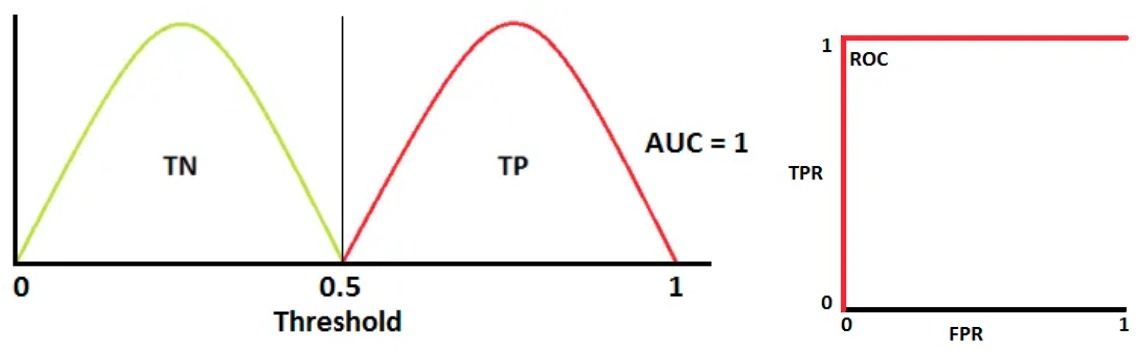
\includegraphics[width=\textwidth]{bilder/auc_1.png}
%     \caption{AUROC = 1.0}
%     \label{fig:auroc_1}
%   \end{minipage}
%   \hfill
%   \begin{minipage}{0.45\textwidth}
%     \centering
%     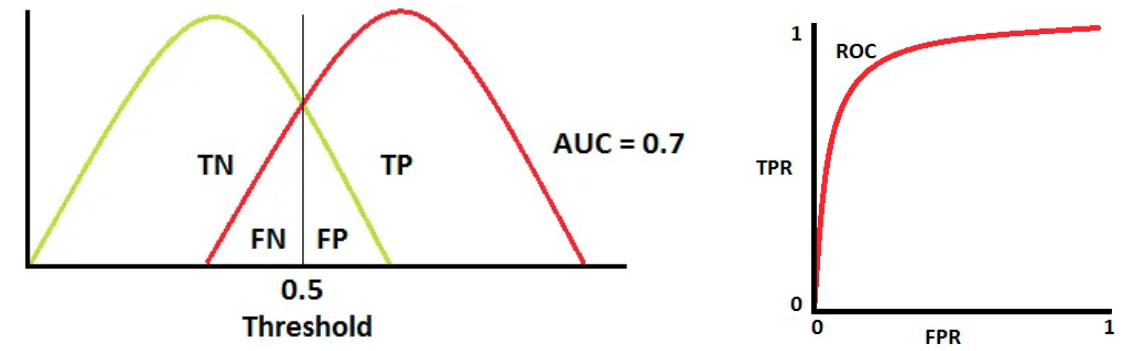
\includegraphics[width=\textwidth]{bilder/auc_07.png}
%     \caption{AUROC = 0.7}
%     \label{fig:auroc_07}
%   \end{minipage}
% \end{figure}

% \begin{figure}[htbp]
%   \centering
%   \begin{minipage}{0.45\textwidth}
%     \centering
%     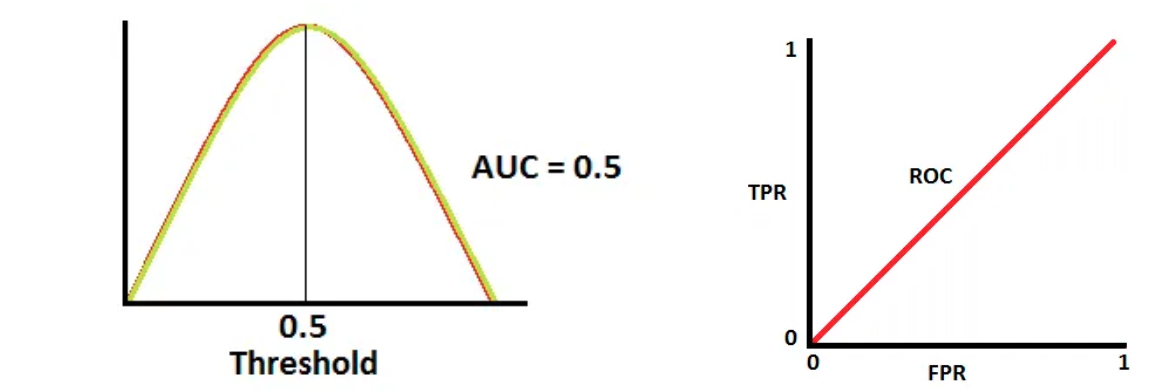
\includegraphics[width=\textwidth]{bilder/auc_05.png}
%     % \caption{AUROC = 0.5}
%     \label{fig:auroc_05}
%   \end{minipage}
%   \hfill
%   \begin{minipage}{0.45\textwidth}
%     \centering
%     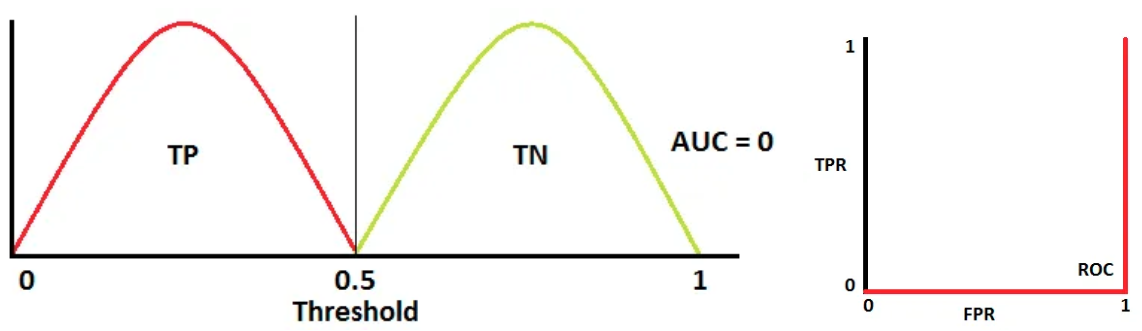
\includegraphics[width=\textwidth]{bilder/auc_0.png}
%     % \caption{AUROC = 0.0}
%     \label{fig:auroc_0}
%   \end{minipage}
% \end{figure}

% \begin{figure}[htbp]
%   \centering
%   \begin{minipage}{0.45\textwidth}
%     \centering
%     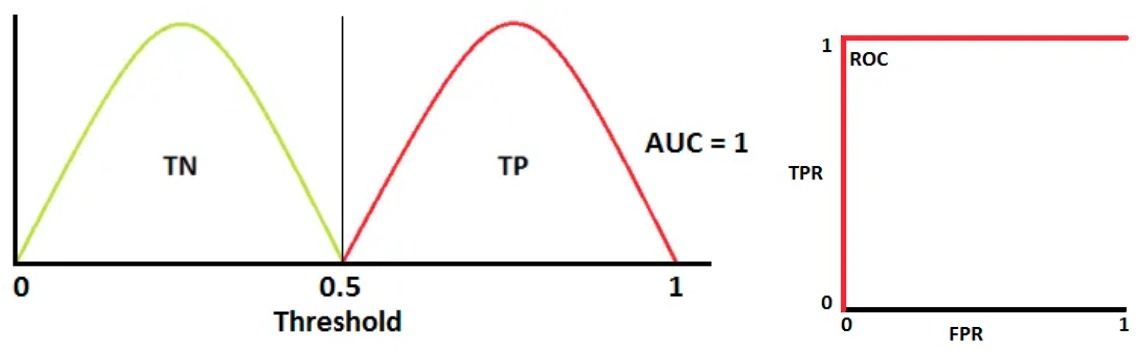
\includegraphics[width=\textwidth]{bilder/auc_1.png}
%     \caption{AUROC = 1.0}
%     \label{fig:auroc_1}
%   \end{minipage}
%   \hfill
%   \begin{minipage}{0.45\textwidth}
%     \centering
%     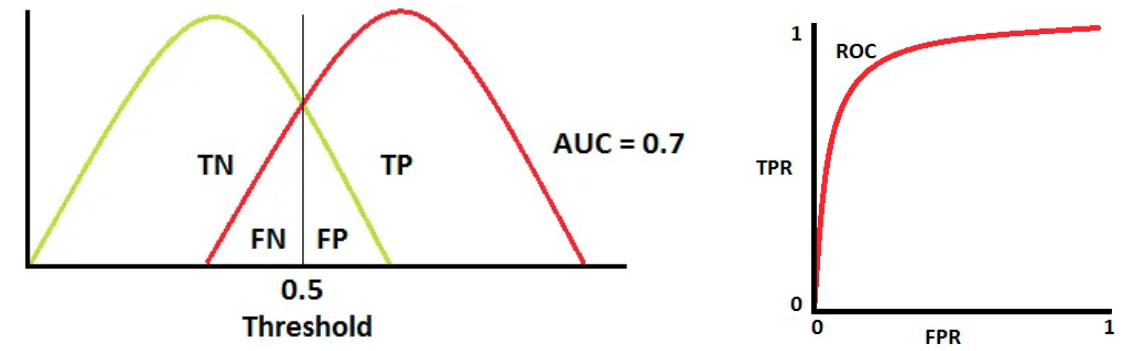
\includegraphics[width=\textwidth]{bilder/auc_07.png}
%     \caption{AUROC = 0.7}
%     \label{fig:auroc_07}
%   \end{minipage}
% \end{figure}

% \begin{figure}[htbp]
%   \centering
%   \begin{minipage}{0.45\textwidth}
%     \centering
%     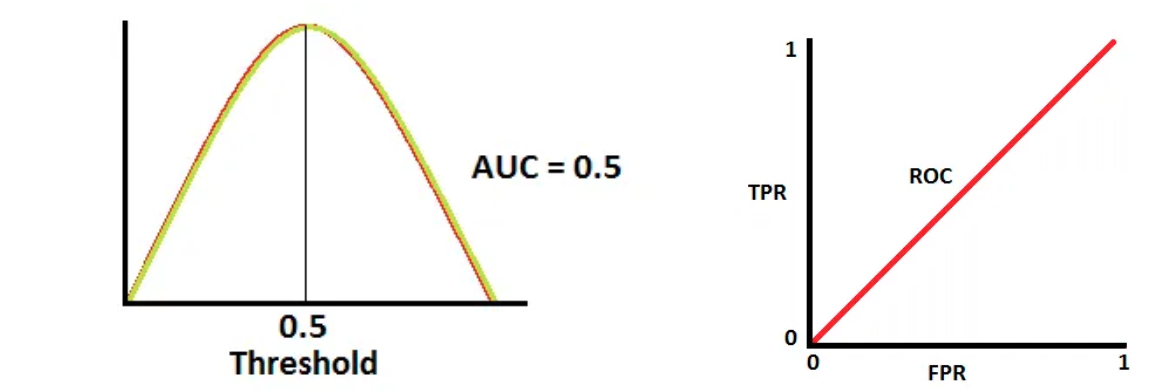
\includegraphics[width=\textwidth]{bilder/auc_05.png}
%     \caption{AUROC = 0.5}
%     \label{fig:auroc_05}
%   \end{minipage}
%   \hfill
%   \begin{minipage}{0.45\textwidth}
%     \centering
%     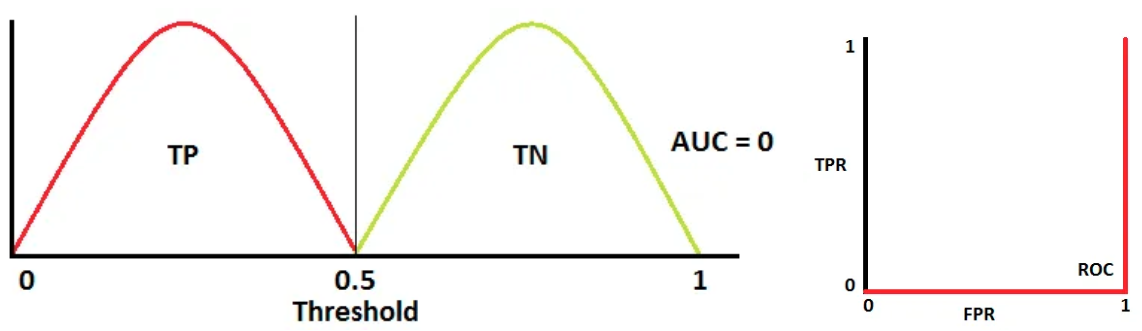
\includegraphics[width=\textwidth]{bilder/auc_0.png}
%     \caption{AUROC = 0.0}
%     \label{fig:auroc_0}
%   \end{minipage}
% \end{figure}


% \begin{figure}[htbp]
%   \centering
%   \begin{minipage}{0.45\textwidth}
%     \centering
%     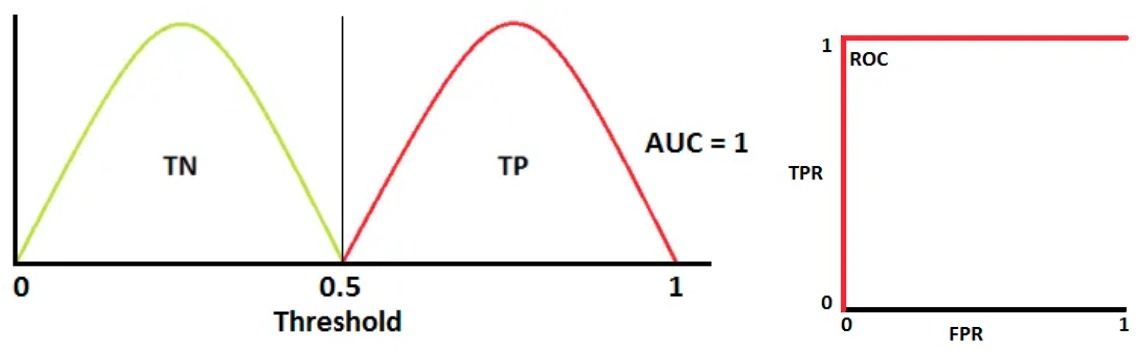
\includegraphics[width=\textwidth]{bilder/auc_1.png}
%     \caption{AUROC = 1.0}
%     \label{fig:auroc_1}
%   \end{minipage}
%   \hfill
%   \begin{minipage}{0.45\textwidth}
%     \centering
%     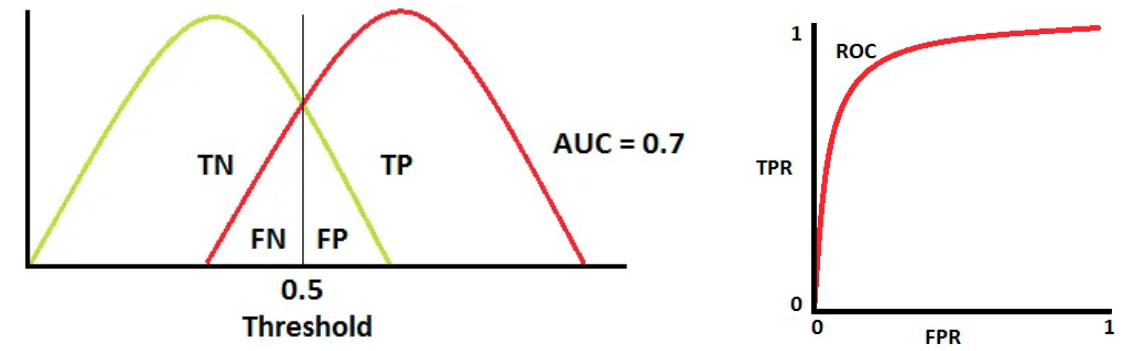
\includegraphics[width=\textwidth]{bilder/auc_07.png}
%     \caption{AUROC = 0.7}
%     \label{fig:auroc_07}
%   \end{minipage}
  
%   \vspace{0.5cm}
  
%   \begin{minipage}{0.45\textwidth}
%     \centering
%     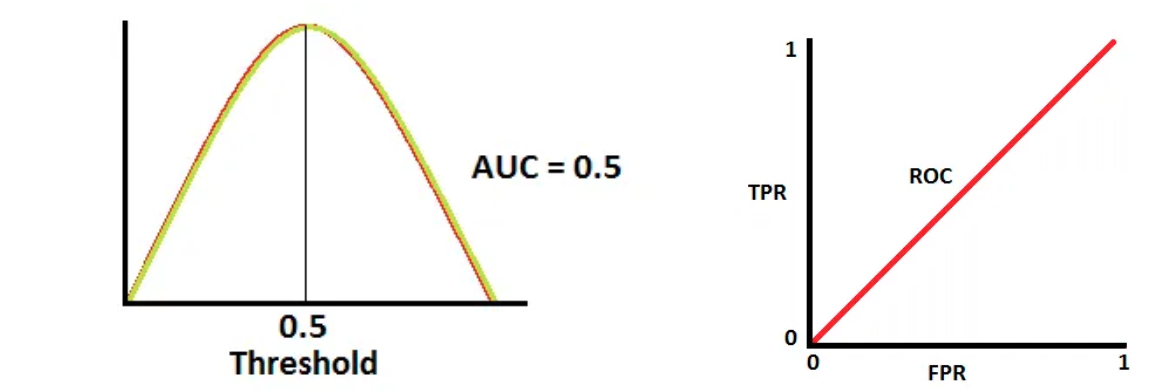
\includegraphics[width=\textwidth]{bilder/auc_05.png}
%     \caption{AUROC = 0.5}
%     \label{fig:auroc_05}
%   \end{minipage}
%   \hfill
%   \begin{minipage}{0.45\textwidth}
%     \centering
%     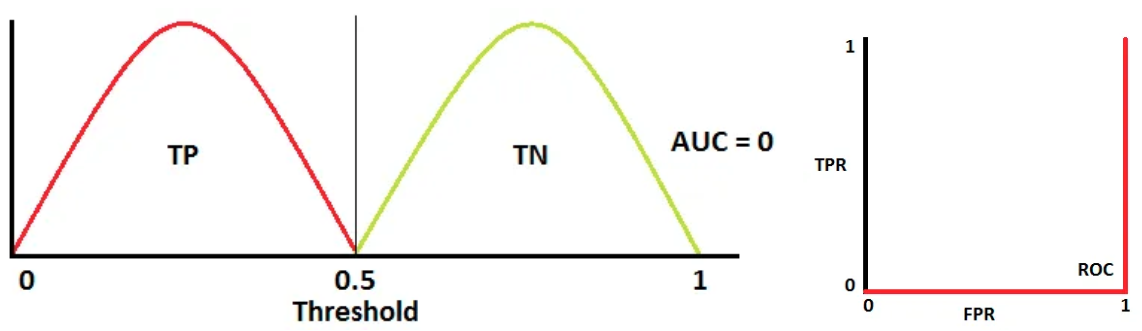
\includegraphics[width=\textwidth]{bilder/auc_0.png}
%     \caption{AUROC = 0.0}
%     \label{fig:auroc_0}
%   \end{minipage}
% \end{figure}
% \end{document}